\documentclass[sigconf,nonacm]{acmart}
\settopmatter{printacmref=false,printfolios=true}
\setcopyright{none}
\renewcommand\footnotetextcopyrightpermission[1]{}
\usepackage{amsmath,tabularx,array,enumitem,balance}
\definecolor{CourseBlue}{HTML}{315EFB}
\definecolor{CourseTeal}{HTML}{14877D}
\hypersetup{colorlinks=true,linkcolor=CourseBlue,citecolor=CourseTeal,urlcolor=CourseTeal}
\newcolumntype{Y}{>{\raggedright\arraybackslash}X}
\setlist{leftmargin=*,topsep=3pt,itemsep=2pt}
\newcommand{\CourseNumber}{COMSCI/ECON 206}
\newcommand{\CourseName}{Computational Microeconomics}
\newcommand{\CourseSession}{Autumn 2026 Session 1}
\newcommand{\Instructor}{Luyao Zhang}
\newcommand{\WorkshopSession}{Workshop 6}
% Replace these with YOUR fork/project URLs, not the instructor's template.
\newcommand{\GitHubLink}{\url{https://github.com/peterhe0616-sketch/PS1-Zhengjun}}
\newcommand{\TemplateRepository}{\url{https://github.com/sunshineluyao/ps1-overleaf-template}}
\newcommand{\ColabLink}{[Insert verified Colab URL]}
\newcommand{\DemoLink}{\url{https://huggingface.co/spaces/Peterhe123/Trust}}
\newcommand{\coursemeta}{\noindent\textbf{Submission to:} \CourseNumber{} --- \CourseName.\\
\textbf{Course session:} \CourseSession. \textbf{Workshop:} \WorkshopSession.\\
\textbf{Instructor:} \Instructor. \textbf{Assignment:} PS1 research proposal.\par\smallskip}
\title{Honesty Through Two-Way Verification: A Credible Disclosure Infrastructure for the Era of Free Generation}
\author{Zhengjun He}
\affiliation{\institution{Duke Kunshan University}\city{Kunshan}\country{China}}
\email{Zhengjun.He@dukekunshan.edu.cn}
\renewcommand{\shortauthors}{Zhengjun He}

\begin{document}
\begin{teaserfigure}
\captionsetup{skip=8pt}
\centering
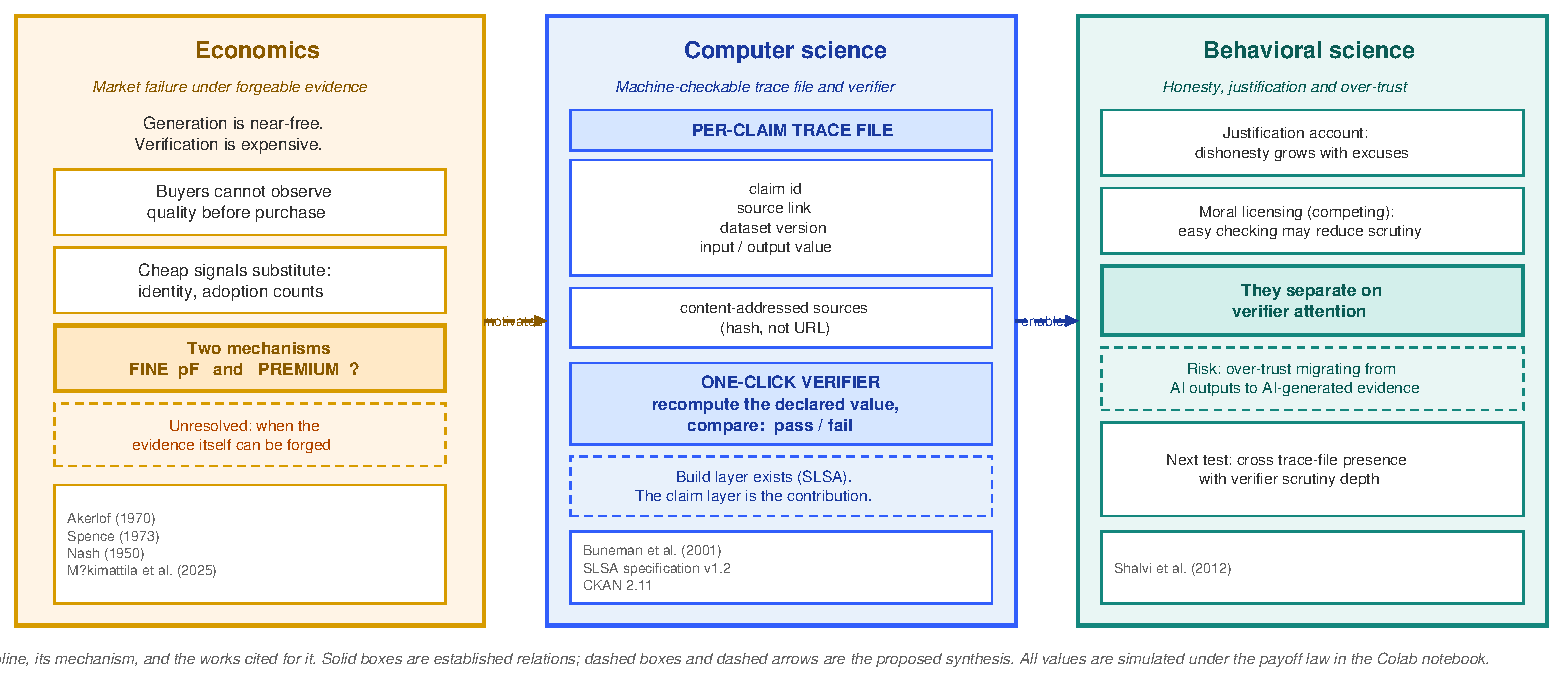
\includegraphics[width=\textwidth]{figures/ps1_teaser.pdf}
\caption{Prospective research design. Three disciplines, one strategic problem, with the works cited for each shown at the foot of its column. Free generation makes fabrication of the documents that carry information nearly costless, so the economic question shifts from what should be disclosed to which rules make honest disclosure stable~\cite{akerlof1970,spence1973,nash1950,makimattila2025}. A machine-checkable per-claim trace file makes a declaration verifiable at near-zero cost, extending the build-layer provenance that already exists~\cite{buneman2001,slsa}. Because effort-free checking may license inattention, the behavioral question is whether traceability shrinks the space for self-serving justification or invites over-trust~\cite{shalvi2012}. Solid boxes are established relations; dashed boxes and dashed arrows are the proposed synthesis. Simulated outcomes, not observations of cognition or markets.}
\Description{A three-column diagram under the headings Economics, Computer science and Behavioral science. The Economics column describes a market where generation is near-free and verification costly, buyers cannot observe quality, and two mechanisms---a fine and a premium---are available, citing Akerlof, Spence, Nash and Makimattila et al. The Computer science column shows a per-claim trace file with content-addressed sources and a one-click verifier, citing Buneman et al., SLSA and CKAN. The Behavioral science column contrasts the justification account against moral licensing and notes the next test, citing Shalvi et al. Dashed arrows labelled motivates and enables connect the three columns. Each column lists its own citations at the foot.}
\label{fig:teaser}
\end{teaserfigure}
\maketitle\raggedbottom\coursemeta

\section{Three connected research questions}
Generating a deliverable, and the documentation meant to vouch for it, is now nearly free while independent verification remains costly. When anyone can fabricate the evidence, the question is not what to disclose but which rules make truthful disclosure stable. The stakeholders are plugin-marketplace developers, the platforms setting the rules, and the users and journalists who act on a claim.

Three foundations frame the problem. Akerlof~\cite{akerlof1970} shows unverifiable quality drives good sellers out of a market. Shalvi et al.~\cite{shalvi2012} show dishonesty grows with available justifications. Buneman et al.~\cite{buneman2001} define provenance as structured lineage, but the producer writes the record, so the trace itself can be forged.

\textbf{Q1---Economics:} Which mechanisms---a fine $pF$ on detected fakes, or a market premium $\Delta$ for verifiable provenance---make honesty a Nash equilibrium when trace files are free to generate and to fake?\par
\textbf{Q2---Computation:} What trace format and verifier make a per-claim declaration checkable at near-zero cost, without trusting the producer's own record?\par
\textbf{Q3---Behavior:} Does traceability shrink the justification space, or does effortless checking produce moral licensing that increases dishonesty?

The three are jointly necessary: a rule requiring trace files is empty unless a fake can be cheaply detected, and an enforceable rule may still fail if checking licenses inattention. Figure~\ref{fig:teaser} connects them.

\section{Answer to Q1: incentives and intellectual lineage}
\textbf{Hypothesis.} Either mechanism suffices. A penalty $pF$ falls only on a detected fake; a premium $\Delta$ is earned only by a verifiable trace file. Honesty is the unique best response when $\Delta + pF$ exceeds the fake's cost advantage.

\textbf{Model.} A developer chooses an action $a_i \in \{\text{honest, none, fake}\}$ and verifier enrolment $v_i \in \{0,1\}$. A platform commits to $(m,p,F)$ for mandatory attachment, spot-check rate and fine; the market sets $\Delta$. Payoff is market benefit plus $\Delta$ if honest, minus cost, plus stability if enrolled, minus $pF$ if faking. A fake earns the same base benefit as an honest deliverable, since buyers cannot observe truth before purchase, while saving cost. Information is incomplete. The solution concept is Nash equilibrium in pure strategies~\cite{nash1950}, with $(m,p,F)$ exogenous; because the platform chooses the rules developers best-respond to, this is a mechanism-design problem.

\begin{table}[h]\caption{Strategy matrix with no rules ($p=F=0$). Left: no premium, so faking wins. Right: a premium, so honesty wins with no enforcement.}\label{tab:matrix}
\renewcommand{\arraystretch}{1.18}
\begin{tabular}{@{}lrr@{}}\toprule
 & \textbf{$\Delta=0$} & \textbf{$\Delta=30$} \\\midrule
A \quad honest trace & 135 & \textbf{165}$^{\star}$ \\
B \quad no trace     & 120 & 120 \\
C \quad faked trace  & \textbf{160}$^{\star}$ & 160 \\\bottomrule
\end{tabular}\end{table}

Without a premium, faking wins by $25$---exactly the cost it avoids---and only a fine can deter it: $p^{*}=0.5$ at $F=50$. With a premium, honesty wins by being worth more. The mechanisms substitute: $\Delta=15$ halves the required spot-check rate to $0.2$, and $\Delta=25$ removes the need to fine at all.

\textbf{Unresolved.} Akerlof fixes buyers' beliefs rather than asking how a costly signal forms them. Spence~\cite{spence1973} supplies that logic: a premium exists only if the signal separates types.

\section{Answer to Q2: method and evaluation}
\textbf{Method.} A browser-run $3\times2$ game on a Hugging Face Space, client-side HTML, CSS and JavaScript; the payoff law is in Appendix~\ref{app:tech}. The algorithm enumerates the six cells and finds the best response.

\textbf{Baseline correction.} The first deployed version summed a cost, a benefit and a stability index. Cost and benefit have opposite signs, so summing them scored honesty as better on both; the sweep returned $p^{*}=0$, meaning faking was never attractive and the question could not be posed. The corrected law enters cost negatively and gives the fake the same benefit as an honest deliverable. See Appendix~\ref{app:develop}.

\textbf{Baseline, modification, metric, check.} Baseline is the status-quo cell (net $120$); the modification is mandatory attachment plus $p$ and $F$; the metric is the threshold $p^{*}$ at which honesty is uniquely best. Six checks pass: no rules $\Rightarrow$ fake wins; enforcement alone makes honesty unique; a premium alone ($\Delta=30$, $p=F=0$) also does; the status quo is unchanged; enrolment is weakly dominant; six cells.

\textbf{Result.} At $F=50$, $p^{*}=0.5000$; the required $p$ falls as $F$ rises ($F=100\Rightarrow0.25$; $F=400\Rightarrow0.0625$), and below $F=25$ no $p\le1$ suffices. All results are \emph{simulated}; the Colab notebook reproduces them from one payoff law.

\section{Answer to Q3: behavior and competing explanations}
\textbf{Competing explanations.} Justification: dishonesty grows with available justifications~\cite{shalvi2012}, so traceability should shrink that space. Moral licensing: a visible attestation lets producer and verifier treat the check as discharging responsibility, so the producer shades a claim the verifier no longer examines. They predict opposite effects from the same manipulation.

\textbf{Discriminating evidence.} They separate on verifier attention. Justification predicts less faking with scrutiny unchanged; licensing predicts reduced scrutiny and a fake rate falling less than the attachment rate rises. Measuring both producer choice and check depth discriminates; measuring the fake rate alone cannot.

\textbf{Consequence and limits.} If licensing dominates, verification must not be a binary pass: it should report which claims were recomputed, and $pF$ must be paired with something keeping scrutiny positive. A simulated table cannot establish human behavior; the next test crosses trace-file presence with check depth.

\section{Advanced development and future directions}
\textbf{Foundation.} Akerlof's quality-uncertainty analysis~\cite{akerlof1970}, recognized by the 2001 Nobel Memorial Prize in Economic Sciences~\cite{nobel2001}, establishes that unverifiable quality destroys markets and that institutions making quality observable restore trade. The enduring question is trust under asymmetric information. Spence~\cite{spence1973} supplies the complementary logic: a costly credible signal separates quality only if the receiver can read it.

\textbf{The boundary and the advance.} Build-layer provenance~\cite{slsa} already exists; unresolved is the claim layer, where per-claim sources and input--output declarations are recomputed at near-zero cost although the producer writes the record and can forge it. Treating $\Delta$ as a constant merely relocates the assumption: a premium exists only if publishing a trace is informative about type, which is Spence's single-crossing condition. If fakers can publish traces as cheaply as honest producers the signal pools, $\Delta$ falls to zero, and enforcement is again the only mechanism. Making $\Delta$ endogenous is the next study; the certification-design result of M{\"a}kimattila et al.~\cite{makimattila2025} is the natural instrument, since there a sender's \emph{choice} among offered tests is itself the signal---but in that model the receiver obtains zero surplus, so a premium does not reach honest producers automatically.

\textbf{The verifier is built for machines.} It returns pass or fail, which a non-specialist cannot interpret; letting an ordinary user judge a firm's claim, or its data-handling practice, is a problem of cognitive rather than computational cost, where the objective is accurate enough and fast enough rather than perfect.

\begin{table}[h]\caption{From laureate foundations to a new interdisciplinary contribution.}
\begin{tabularx}{\columnwidth}{@{}p{1.5cm}Y@{}}\toprule
\textbf{Horizon}&\textbf{Milestone and evidence}\\\midrule
Foundation&Akerlof (1970): unverifiable quality collapses markets. Spence (1973): a credible signal needs single crossing.\\
PS1&A $3\times2$ game; two mechanisms located, a fine $pF$ and a premium $\Delta$, with $\Delta+pF>25$ required.\\
Next study&Endogenise $\Delta$ in buyer beliefs: does trace publication separate types or pool?\\
Longer term&A verifier a non-specialist can use, reporting what was checked, at what accuracy and cost.\\
2056&Verifiable honesty that is competitively rewarded, not merely enforced, and readable by any user.\\\bottomrule
\end{tabularx}\end{table}

\noindent\textbf{Expected 2056 Nobel Prize and Turing Award contribution statement.}
By 2056, I aim to contribute a governed trust infrastructure for an era of free generation, in which verifiable provenance is competitively rewarded rather than merely enforced, and in which any ordinary user can check a firm's claims and data-handling practices without technical training. Building on Akerlof's quality-uncertainty foundation, Spence's signalling logic and machine-checkable provenance, I will integrate economics, computer science and behavioral science so that near-zero-cost trace files, a verifier designed for non-specialists, and platform rules that make honest publication an equilibrium together let anyone inspect a claim in under a minute. Progress will be shown by an endogenous premium that separates honest from faking producers, a verifier whose accuracy and cost are documented, a discriminating behavioral test, and a rule design adopted on a live platform.

\subsection*{Open Science Statement}
\textbf{GitHub:} \GitHubLink\\
\textbf{Google Colab:} \ColabLink\par
Released: a browser-run simulator and a Colab notebook that re-derives the payoff table and runs both sweeps. The simulator is static client-side HTML/CSS/JavaScript with no backend or key; the notebook needs only Python. Inputs are synthetic: one payoff law read by both. Shortest run: open the notebook and choose \emph{Run all}.

\subsection*{Statement of Contribution to the UN's SDGs}
\textbf{Hugging Face:} \DemoLink\\
Through an open-access game, this project supports \textbf{SDG 4---Quality Education}~\cite{sdg4} by helping students and the public learn why honest disclosure requires cheap verification, by comparing the six rule-and-action combinations. No account or installation is needed. The resource released is the simulator; learning gains remain to be evaluated.

\subsection*{Submission milestones}
This is v1, submitted September 13, 2026, 11:00 P.M. Beijing time (UTC+8). Class review: September 14. Author response: September 16. Reviewer follow-up: September 17. Revised submission v2: September 20. Appendix~\ref{app:abstract} records each reflection and revision; row~8 is marked pending, as no peer review has been received.

\clearpage\nobalance
\section*{Author Notes}
\subsection*{Acknowledgements}
I thank Prof. Luyao Zhang, Program Chair, and Prof. Ken Rogerson, Program Discussant, of the \emph{2056 Nobel and Turing Laureate Program Launch Workshop}, Duke Kunshan University, September 7, 2026; Longfei Jing and Yongzhuo Wu, my teammates in Workshop 6; and the rest of the COMSCI/ECON 206 Autumn 2026 Session 1 class. I am responsible for the proposal and remaining errors.
\subsection*{Individual contribution}
I formed the core idea, posed the research question, and developed the one-click verifier, the lemons-market framing and the rule triple $(m,p,F)$. I verified the literature, played the game, and on 9 September found and corrected two errors in the payoff law (Appendix~\ref{app:develop}). The photographs, the numbers and the final wording are mine.

\bibliographystyle{ACM-Reference-Format}\bibliography{references}
\appendix
\section{Technical details and reproducibility}\label{app:tech}
\textbf{Notation.} $a_i$ developer $i$'s action (honest, none, fake); $v_i$ verifier enrolment; $m$ mandatory attachment; $p$ spot-check rate; $F$ fine on a detected fake; $pF$ expected fine; $\Delta$ premium paid only for a verifiable trace file; $p^{*}$ smallest $p$ making honesty the unique best response.

\textbf{Artifact.} Trace-or-Fake Market Game, a $3\times2$ simulator. Space: \url{https://huggingface.co/spaces/Peterhe123/Trust}. Notebook: \texttt{colab/trace\_or\_fake\_psweep.ipynb}. Author: Zhengjun He. v1.0.0, 6 September 2026.

\textbf{Payoff law.} A developer chooses honest, none or fake, and whether to enrol in the verifier. Payoff is market benefit plus $\Delta$ if honest, minus cost, plus stability if enrolled, minus $pF$ if faking. A fake earns the same base benefit as an honest deliverable, since buyers cannot observe truth before purchase, while saving cost.

\textbf{Corrections, 9 September 2026.} (i) The first law summed a cost, a benefit and a stability index. Cost and benefit have opposite signs, so summing them scored honesty as better on both before any rule applied, and the sweep returned $p^{*}=0$: faking was never attractive, so the question could not be posed. Cost now enters negatively. (ii) Honest and faked traces were then paid identically, so honesty won only by avoiding a penalty. A premium $\Delta$ paid only for a verifiable trace file repairs this; the two mechanisms substitute, giving $\Delta+pF>25$ against a fake advantage of $25$. At $\Delta=0$, $p^{*}=0.5$ at $F=50$; at $\Delta=15$, $p^{*}=0.2$; at $\Delta=25$, no enforcement is needed.

\textbf{Fresh-run record.} Python 3.11, standard library only, deterministic, no seed needed. Six checks pass: no-rules fake wins; enforcement alone makes honesty unique; a premium alone ($\Delta=30$) also does; status quo unchanged; enrolment weakly dominant; six cells. Abridged output:

\begin{quote}\small\ttfamily
no rules: A 135, B 120, C 160  ->  best response C\_fake\\
threshold p* = 0.5000 (F = 50);  F=100 -> 0.2500;  F=400 -> 0.0625\\
premium sweep (p=F=0): 0 -> C\_fake;  25 -> tie;  30 -> A\_honest\\
combined: delta=0 -> p*=0.50;  delta=15 -> p*=0.20;  delta=25 -> no enforcement
\end{quote}

\textbf{Boundary.} Static client-side HTML/CSS/JavaScript only: no runtime, backend, key or paid service. Hosting and the viewer's browser still consume energy~\cite{lannelongue2021}. Semantic fieldsets, table captions and keyboard operability are present; a full screen-reader pass is unverified. The deployed Space should be updated to the corrected law.

\subsection{AI-use disclosure}
I completed all substantive work myself: the research question, the payoff law, the strategy matrix, the two corrections to that law, the derivation of the threshold $\Delta+pF>25$, the computational checks, the game, the notebook and the argument of the paper. Every source was read and every number re-derived by me, and I played the game and ran the checker. A generative AI assistant (DeepSeek, model \texttt{deepseek-v4-flash}, accessed 6 September 2026) was used only for \LaTeX{} typesetting and layout, and for brainstorming possible literature to look up. It did not devise the model, run any computation, or write the argument. All literature it suggested was independently located and verified before citation. Initial reasoning and handwritten reflection are Human-Only, and I remain responsible for every claim.

\section{Cumulative Intellectual Development}\label{app:develop}
This proposal develops my Intellectual Statement II through the \emph{2056 Nobel and Turing Laureate Program Launch Workshop}, September 7, 2026, Duke Kunshan University, IB 2050. Program Chair: Prof. Luyao Zhang. Program Discussant: Prof. Ken Rogerson. My session: Workshop 6. My role: Computer scientist. My teammates: Longfei Jing and Yongzhuo Wu.

\textbf{First change: the object of the question.} My earlier claim was that I would build mechanisms letting agents cooperate under near-total unobservability. The September 4 evidence forced something narrower: at the Tencent Shanghai Office plugin quality is hard to observe before adoption, and at the Shanghai Science and Technology Museum the deep-residual-learning panel asks a general audience to trust institutional authority rather than checkable evidence. The marketplace is a market without institutional trust; the museum is institutional trust without a market. Workshop feedback sharpened the boundary---build-layer provenance already exists, so the contribution must sit at the claim layer---moving the proposal from a disclosure design to a rule design.

\textbf{Second and third changes, 9 September 2026.} The notebook sweep returned $p^{*}=0$, showing the game summed cost with the wrong sign, so honesty won regardless of any rule and the game could not pose its own question. With that fixed, honest and faked traces were still paid identically, so honesty was a tax rather than an asset. Reading M{\"a}kimattila et al.~\cite{makimattila2025}, where a sender's \emph{choice} among offered tests is itself informative, together with Spence's single-crossing condition~\cite{spence1973}, prompted adding the premium $\Delta$. The proposal can now show honesty wins because it is worth more, not merely because cheating is punished. What remains unresolved: $\Delta$ is still a parameter rather than a belief, so making it endogenous is the next study.

\section{Field and open-source inspiration}
The \emph{Joint Interdisciplinary Field Trip---Technology, Computation, Culture \& Society in Action} took place on September 4, 2026.

\textbf{Tencent Shanghai Office.} Observation: WorkBuddy is Tencent's AI agent platform, whose marketplace connects plugin developers with users. Interpretation: plugin quality is hard to observe before adoption, so buyers rely on cheap signals, and costly verification can produce a lemons market. Photograph: \emph{WorkBuddy agent-plugin marketplace}, by the author, 4 September 2026.

\textbf{Shanghai Science and Technology Museum.} Observation: the 2023 Mathematics and Computer Science Prize panel~\cite{futureprize2023} presents deep residual learning through simplified diagrams. Interpretation: trust here rests on institutional authority, not on independently checkable evidence. Photograph: \emph{2023 Mathematics and Computer Science Prize panel}, by the author, 4 September 2026.

\textbf{Two open-source tools.} (i) \emph{SLSA}~\cite{slsa}, \url{https://slsa.dev/}, v1.2, Apache-2.0: generates non-forgeable build provenance, so a verifier can check which commit built which artifact, but certifies the build chain only, not whether the artifact does what its description claims. (ii) \emph{CKAN}~\cite{ckan}, \url{https://ckan.org/}, 2.11, AGPL-3.0: an open-data catalog with standardised metadata and public APIs that stores whatever publishers upload and never checks whether a dataset matches its description. Consequence: SLSA supplies the build layer at near-zero cost and CKAN the public substrate, so my contribution is the claim layer both ignore.

\section{Review response and revision record}
No peer review has been received as of v1. In-class review is September 14, 2026; no reviewer feedback is claimed. This section will be completed with the author response and the v2 revision.

\clearpage\onecolumn
\section{Structured abstract and cumulative proposal map}\label{app:abstract}
\par\medskip
\begin{table}[H]
\caption{Appendix E structured abstract; the eight-row proposal structure.}
\label{tab:abstract-map}
\renewcommand{\arraystretch}{1.18}
\begin{tabularx}{\textwidth}{@{}p{0.27\textwidth}Y@{}}
\toprule
\textbf{Proposal element} & \textbf{Current statement} \\
\midrule
Background & Build-layer traceability already exists and generation is near-free, while unchecked quality uncertainty collapses markets. Foundations: Akerlof (1970); Buneman et al. (2001). \\
Motivation and application & Untested: which mechanisms make honest trace files an equilibrium when they are free to generate and to fake. Scenario: a plugin marketplace setting the rules, with users and journalists as verifiers; it scales to public claims. \\
Three connected questions & Economics: does a fine $pF$ or a premium $\Delta$ make honesty a Nash equilibrium? Computation: what format and verifier make a per-claim declaration checkable at near-zero cost? Behavior: does traceability shrink the justification space, or does easy checking license less scrutiny? Integrated: which rules make honest disclosure stable when the evidence can be forged? \\
Method and model assumptions & Developers choose honest, none or fake, plus enrolment; the platform commits to $(m,p,F)$ and the market sets $\Delta$. Information is incomplete. Payoff is benefit plus $\Delta$ if honest, minus cost, plus stability if enrolled, minus $pF$ if faking; a fake earns the same base benefit as an honest deliverable. Baseline nets $120$; the computation is a $3\times2$ enumeration plus sweeps of $p$ and $\Delta$. \\
Results & Verified: with no rules and $\Delta=0$ the fake wins ($160$ vs $135$); a premium alone restores honesty, and without one honesty requires $pF>25$ ($p^{*}=0.5000$ at $F=50$). The two substitute: $\Delta=15$ gives $p^{*}=0.20$; $\Delta=25$ needs no enforcement. Six checks pass. Evidence type: simulated, from one shared payoff law. Two corrections; see Appendix~\ref{app:develop}. \\
Intellectual merits & Checkability becomes an institutional variable rather than a technical property, extending lemons theory to claims under free generation, where the certification instrument is itself forgeable. Separating enforcement from reward and showing they are substitutes reframes the design problem from policing to pricing. \\
Practical impacts & Private: lower screening costs on plugin and agent platforms. Public: auditable claims in museums, ministries and data portals. The SDG 4 tool lets students and the public learn why honest disclosure needs cheap verification, assessable by a short pre/post prediction question. The simulator is released; learning gains remain unevaluated. \\
Feedback received and revision made & September 7 workshop feedback established that build-layer provenance already exists, moving the contribution to the claim layer and revising the 2056 statement from cooperation under unobservability to a governed trust infrastructure. September 9, two dated changes: the sweep returned $p^{*}=0$, exposing a sign error; and reading M\"akimattila et al.~\cite{makimattila2025} showed honesty was modelled as a cost rather than an asset, so a premium $\Delta$ was added. Peer reviews pending; none claimed. \\
\bottomrule
\end{tabularx}
\end{table}

\end{document}
